\documentclass{article}
\usepackage[T1]{fontenc}
\usepackage{graphicx}
\usepackage{tcolorbox} % Pakiet do ramek
\usepackage{lmodern}
\usepackage{amsmath}
\usepackage[MeX]{polski}
\usepackage{geometry}
\usepackage[MeX]{polski}
\usepackage{float}
\geometry{a4paper}

\title{System rekomendacyjny wypożyczalni filmów z rozmytością}

\author{\textbf{Raport końcowy} \\ \\ Piotr Iśtok \\ Piotr Jacak}
\date{Czerwiec 2025}

\begin{document}

\maketitle


\tableofcontents
\newpage

\section{Dane}
Dane do omawianego systemu rekomendacyjnego zostały pobrane ze strony https://grouplens.org/datasets/movielens/. Zbiór danych zawiera trzy pliki:
\begin{itemize}
    \item \textit{movies.csv} - tabela z kolumnami: identyfikator filmu, tytuł filmu, gatunek filmu (gatunki wypisane obok siebie, oddzielone znakiem '|').
    \item \textit{tags.csv} - tabela z kolumnami: identyfikator użytkownika dodającego tag, identyfikator filmu, tag, znacznik czasowy dodania tagu.
    \item \textit{ratings.csv} - tabela z kolumnami: identyfikator użytkownika, identyfikator filmu, ocena (w skali od $0$ do $5$), znacznik czasowy dodania oceny. 
\end{itemize}

\section{Eksploracyjna Analiza Danych - EDA}
\subsection{Cel i zakres analizy}
Celem eksploracyjnej analizy danych było lepsze zrozumienie struktury, rozkładu i jakości danych wejściowych oraz identyfikacja potencjalnych problemów, które mogłyby wpłynąć na skuteczność systemu rekomendacyjnego. Analiza objęła trzy podstawowe źródła danych: oceny użytkowników (\textit{ratings.csv}), informacje o filmach (\textit{movies.csv}) oraz przypisane tagi (\textit{tags.csv}).

\subsection{Struktura zbioru danych}
\begin{itemize}
    \item Liczba ocen: 32000204
    \item Liczba użytkowników: 200948
    \item Liczba unikalnych filmów: 87585
    \item Liczba tagów: 140979
\end{itemize}

\subsection{Rozkład ocen}
Rozkład ocen użytkowników jest asymetryczny, z przewagą ocen pozytywnych – najwięcej ocen znajduje się w przedziale 3.0–4.0. Średnia ocena wynosi 3.54, a mediana to 3.5, co sugeruje umiarkowanie pozytywne nastawienie użytkowników do ocenianych filmów.
\begin{figure}[H]
\centering
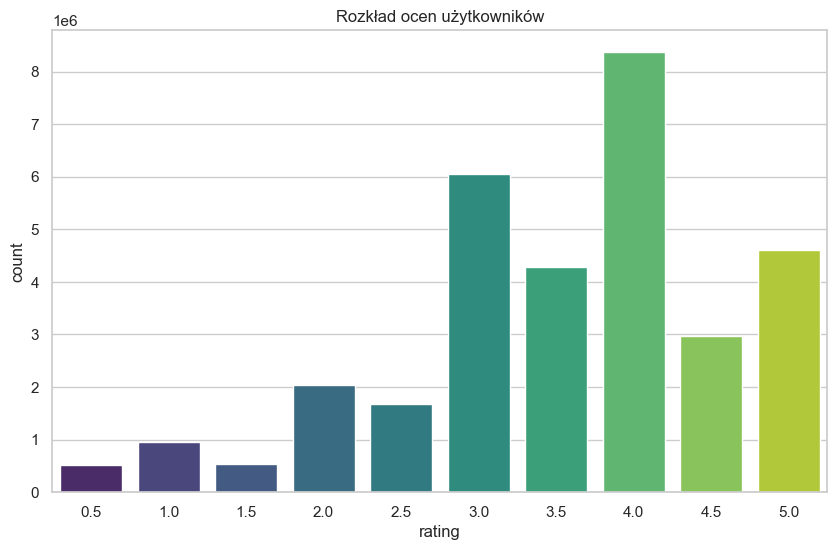
\includegraphics[width=1\textwidth]{pictures/oceny_rozklad.png}
\caption{Rozkład ocen użytkowników}
\label{fig:oceny_rozklad}
\end{figure}


\subsection{Aktywność użytkowników i popularność filmów}
\begin{itemize}
    \item Średnia liczba ocen na użytkownika: 159.25
    \item Mediana liczby ocen na użytkownika: 73
    \item Najwięcej ocen użytkownika: 33332
    \item Najmniej ocen użytkownika: 20
\end{itemize}
Następnie został jeszcze zbadany rozkład liczby ocen na film. Wyniki są pokazane poniżej.
\begin{figure}[H]
\centering
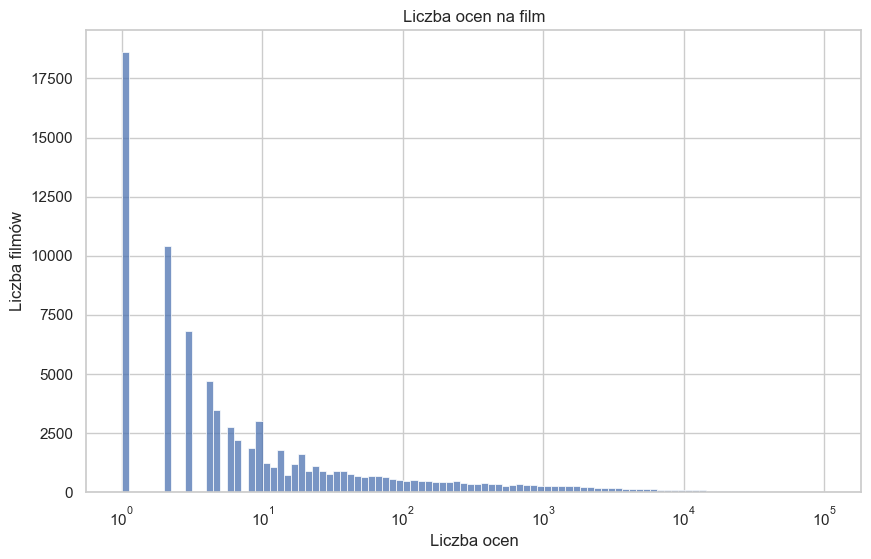
\includegraphics[width=1\textwidth]{pictures/locen_per_film.png}
\caption{Rozkład liczby ocen filmów}
\label{fig:oceny_per_film_rozklad}
\end{figure}
Rozkład liczby ocen na użytkownika i na film ukazuje typową sytuację dla systemów rekomendacyjnych – nieliczni użytkownicy są bardzo aktywni, a nieliczne filmy bardzo popularne.

\subsection{Gatunki filmów}
W analizie uwzględniono zarówno surowe liczenie przynależności filmu do gatunku (bez wag), jak i podejście z uwzględnieniem proporcji, gdy film należy do wielu kategorii. Najczęściej występujące gatunki to: Drama, Comedy i Thriller. Poniżej pokazano wykres rozkładu liczby filmów o danym gatunku.

\begin{figure}[H]
\centering
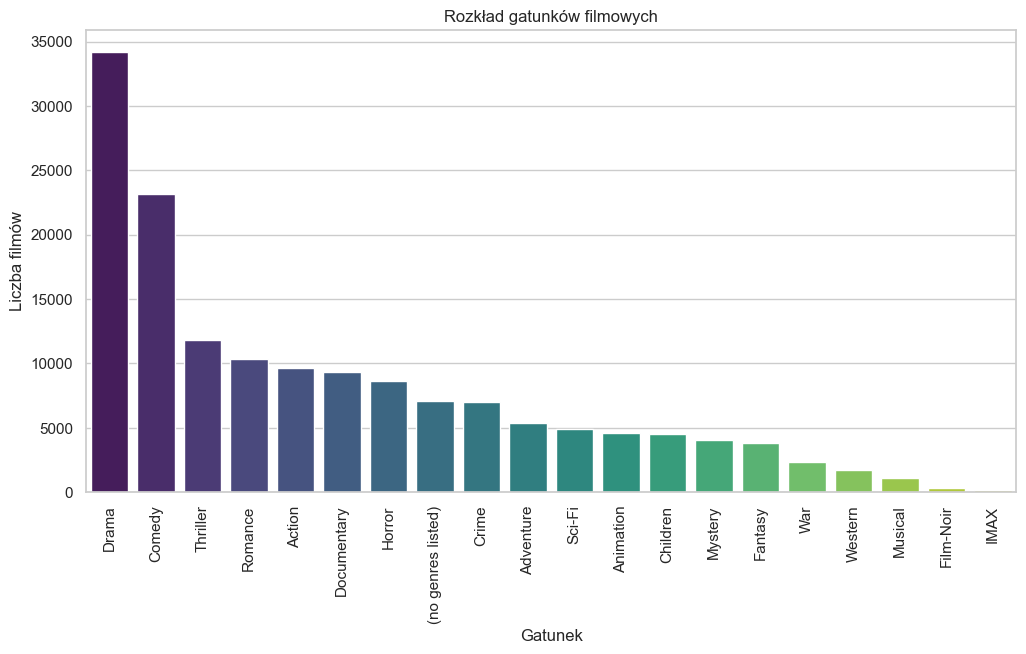
\includegraphics[width=1\textwidth]{pictures/rozklad_gatunku_filmow.png}
\caption{Rozkład gatunków filmów}
\label{fig:rozklad_gatunkow}
\end{figure}
Została następnie wyznaczona mediana, wartość maksymalna oraz obliczona średnia liczba gatunków na film.
\begin{itemize}
    \item Mediana liczby gatunków na film: 1
    \item Maksymalna liczba gatunków filmu: 10
    \item Średnia liczba gatunków na film: 1.76
\end{itemize}
W drugim wariancie przyjęliśmy, że przynależność filmu do gatunku filmowego będzie dzielona przez ilość wszystkich gatunków, do których należy. W takim przypadku oczywiście nie ma sensu badania średniej, wartości maksymalnej oraz mediany ilości gatunków filmu, bo wynoszą one 1.
\begin{figure}[H]
\centering
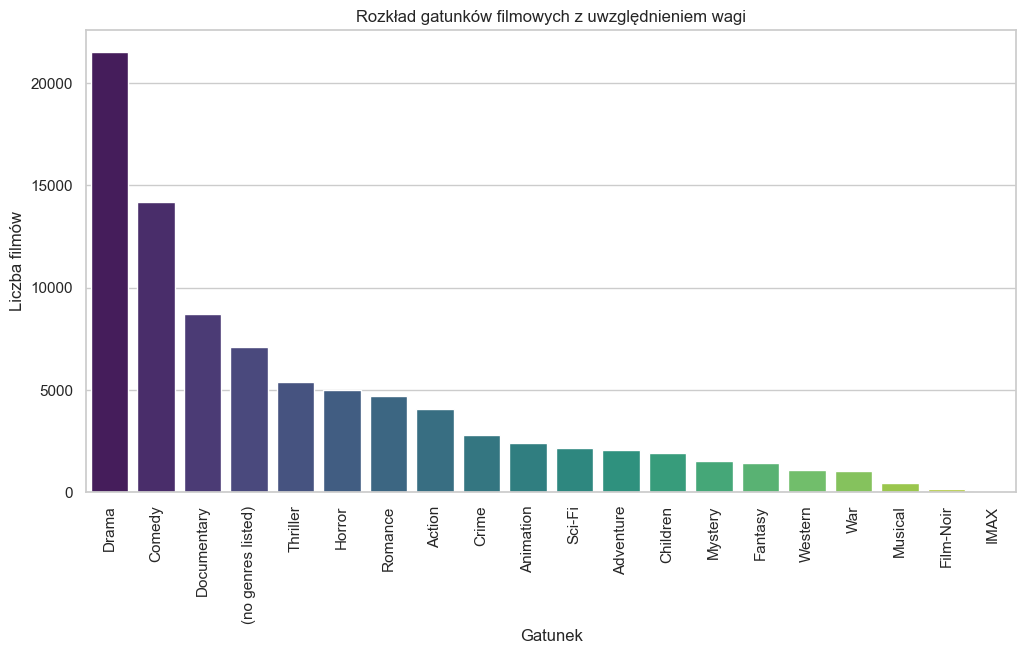
\includegraphics[width=1\textwidth]{pictures/rozklad_gatunku_filmow_weighted.png}
\caption{Rozkład gatunków filmów wyważona w zależności od ilości gatunków, do których należy}
\label{fig:rozklad_gatunkow}
\end{figure}
Można zauważyć, że znaczenie gatunku Thrille spada i znajduję się już tylko na 5 miejscu i jego 3 miejsce zajmuje gatunek Documentary.
\subsection{Analiza jakościowa filmów}
Dla każdego gatunku obliczono średnią ocenę. Najwyżej oceniane były m.in. filmy z gatunków takich jak: Film-Noir i Documentary. Taka analiza wspiera dobór cech do części content-based modelu.
\begin{figure}[H]
\centering
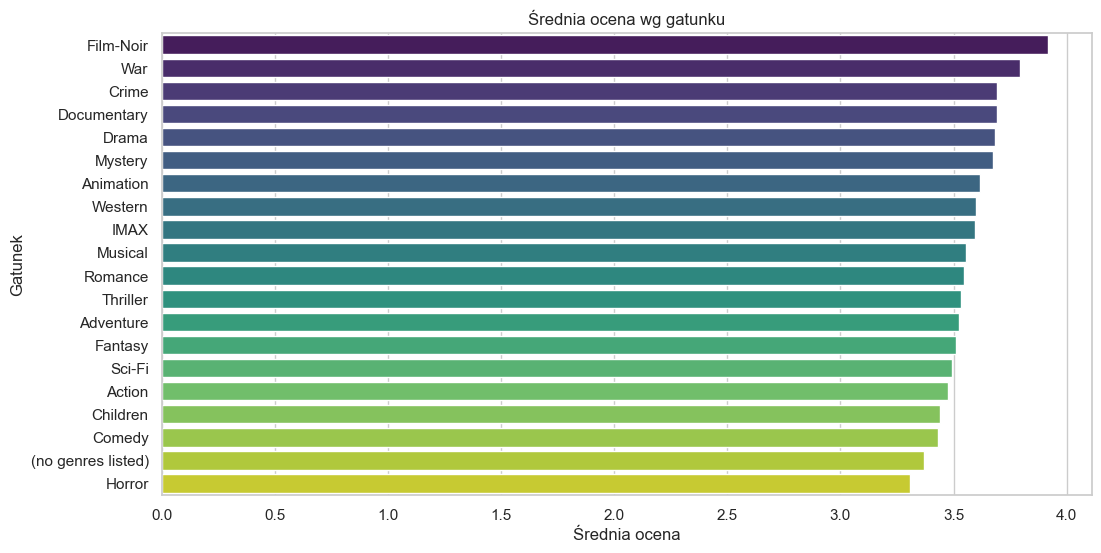
\includegraphics[width=1\textwidth]{pictures/mean_ocena_wg_gatunku.png}
\caption{Średnia ocena według gatunku, do którego należy film}
\label{fig:mean_ocena_wg_gatunku}
\end{figure}

\subsection{Analiza tytułów filmów}
Z tytułów wydobyto lata produkcji oraz najczęstsze słowa – zarówno przed, jak i po oczyszczeniu (usunięcie stopwords i lematyzacja). Celem tego etapu było stworzenie efektywnych cech tekstowych do modelu content-based filtering.

\begin{figure}[H]
\centering
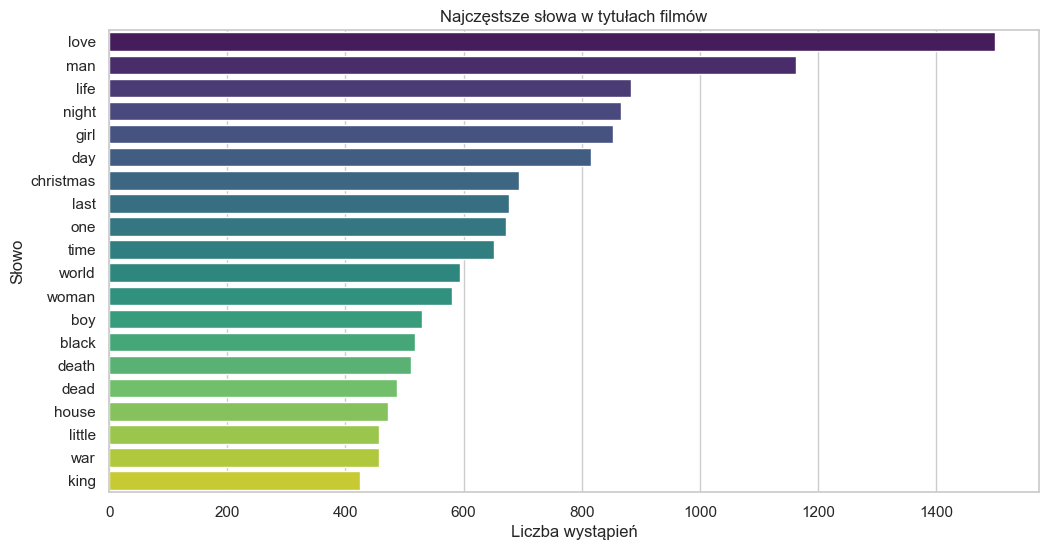
\includegraphics[width=1\textwidth]{pictures/most_often_used_words.png}
\caption{Najczęstsze słowa w tytułach filmów}
\label{fig:most_often_used_words}
\end{figure}

\subsection{Wnioski}
Eksploracja danych pozwoliła:
\begin{itemize}
    \item potwierdzić przydatność danych wejściowych do dalszego modelowania,
    \item wskazać potencjalne ograniczenia,
    \item przygotować odpowiednie cechy dla obu komponentów systemu rekomendacyjnego.
\end{itemize}
\section{Content-based filtering}
Poniżej przedstawiono sposób implementacji metody content-based filtering w omawianym systemie rekomendacyjnym.
\begin{enumerate}
    \item Za pomocą biblioteki \textit{pandas} wczytano tabele z plików \textit{csv}. 
    \item Pogrupowano tabelę \textit{tags} i połączono wszystkie tagi dla danego filmu w jedną komórkę tabeli.
    \item Połączono tabele \textit{tags} oraz \textit{movies} na podstawie identyfikatora filmu. Stworzono połączony wektor zawierający wszystkie tagi oraz gatunki dla danego filmu, oddzielone spacją.
    \item Z biblioteki \textit{scikit-learn} wykorzystano funkcję \textit{TfidVectorizer}. Funkcja tworzy macierz, gdzie wiersze to poszczególne filmy, natomiast kolumny to słowa występujące w wektorach utworzonych wyżej (funkcja bierze pod uwagę tylko te słowa, które wystąpiły co najmniej dwa razy i pomija spójniki w języku angielskim). Wartości w macierzy to wartości $TF-IDF$. \\ 
    Wartość $TF-IDF$ to iloczyn wartości $TF$ i $IDF$, gdzie:
    \begin{itemize}
        \item $TF$:
        \begin{equation}
            tf_{i,j} = \frac{n_{i, j}}{\sum_k n_{k, j}}
        \end{equation}
        gdzie $n_{i,j}$ jest liczbą wystąpień słowa dla danego filmu, a mianownik jest sumą liczby wystąpień wszystkich słów dla danego filmu.
        \item $IDF$:
        \begin{equation}
            idf_i = log \frac{|D|}{|\{d:t_i \in d\}|}
        \end{equation}
        gdzie $|D|$ to liczba filmów, a $|\{d:t_i \in d\}|$ - liczba filmów zawierających przynajmniej jedno wystąpienie danego słowa. 
    \end{itemize}
    \item Rekomendacja dla danego użytkownika
    \begin{itemize}
        \item Zbudowanie profilu użytkownika: z macierzy $TF-IDF$ stworzenie wektora filmów, które użytkownik ocenił powyżej $4$ - wartości w takim wektorze to średnia wartości w macierzy dla danego filmu.
        \item Obliczenie podobieństwa cosinusowego między wektorem użytkownika a całą macierzą $TF-IDF$. Podobieństwo jest w skali $[0,1]$ co przekłada się na rozmytość - \textbf{film może tylko w pewnym stopniu przynależeć do zbioru polecanych filmów}
        \item Wybranie filmów nieobejrzanych przez użytkownika i tych z najwyższą wartością podobieństwa.
    \end{itemize}
\end{enumerate}

\section{Collaborative filtering}
Poniżej przedstawiono sposób implementacji metody collaborative item-item filtering w omawianym systemie rekomendacyjnym.
\begin{enumerate}
    \item Za pomocą biblioteki \textit{pandas} wczytano tabele z plików \textit{csv}. 
    \item Przy pomocy biblioteki \textit{scipy} stworzony macierz rzadką \textit{użytkownik-film}.
    \item Przeskalowano oceny, tak aby różnicę między ocenami były większe.
    \item Wykorzystanie funkcji Okapi BM25 w celu wyważenia wpływu bardzo popularnych filmów, które mogłyby dominować podobieństwa.
    \item Przy pomocy biblioteki \textit{implicit} wyznaczenie macierzy podobieństwa cosinusowego przy zapamiętaniu tylko k-najbliższych sąsiadów (w naszym wypadku 500).
    \item Rekomednacje:
    \begin{enumerate}
        \item Dla istniejącego użytkownika w modelu: \textit{model.recommend()}.
        \item Dla pojedynczego filmu: \textit{model.similar\_items()}.
        \item Dla nowego użytkownika: stworzenie ręcznego wektora ocen, użycie macierzy podobieństwa \textit{model.similarity} i samodzielne obliczenia
    \end{enumerate}
\end{enumerate}
\section{System hybrydowy}
Poniżej przedstawiono implementację finalnego systemu hybrydowego, w omawianym systemie eksperckim:
\begin{enumerate}
    \item Zarekomendowanie 2000 najbardziej wskazanych filmów dla danego użytkownika przy użyciu metody CBF oraz 2000 filmów przy użyciu metody CF.
    \item Wartości podobieństwa ($[0,1]$) uzyskane za pomocą metody CF zostały pomnożone przez $0,6$, natomiast wartości podobieństwa uzyskane za pomocą metody CBF przez $0,4$ - średnia ważona uwzględniająca lepsze wyniki otrzymywane w ogólności przez CF.
    \item Posortowanie otrzymanych wartości podobieństwa i zwrócenie filmów, dla których końcowe wartości podobieństwa są najwyższe.
\end{enumerate}

\section{Przykładowa rekomendacja}
Poniżej na rysunku \ref{fig:results} znajduje się przykładowa rekomendacja dziesięciu filmów przy użyciu systemu hybrydowego dla użytkownika o ID 5.
\begin{figure}[H]
\centering
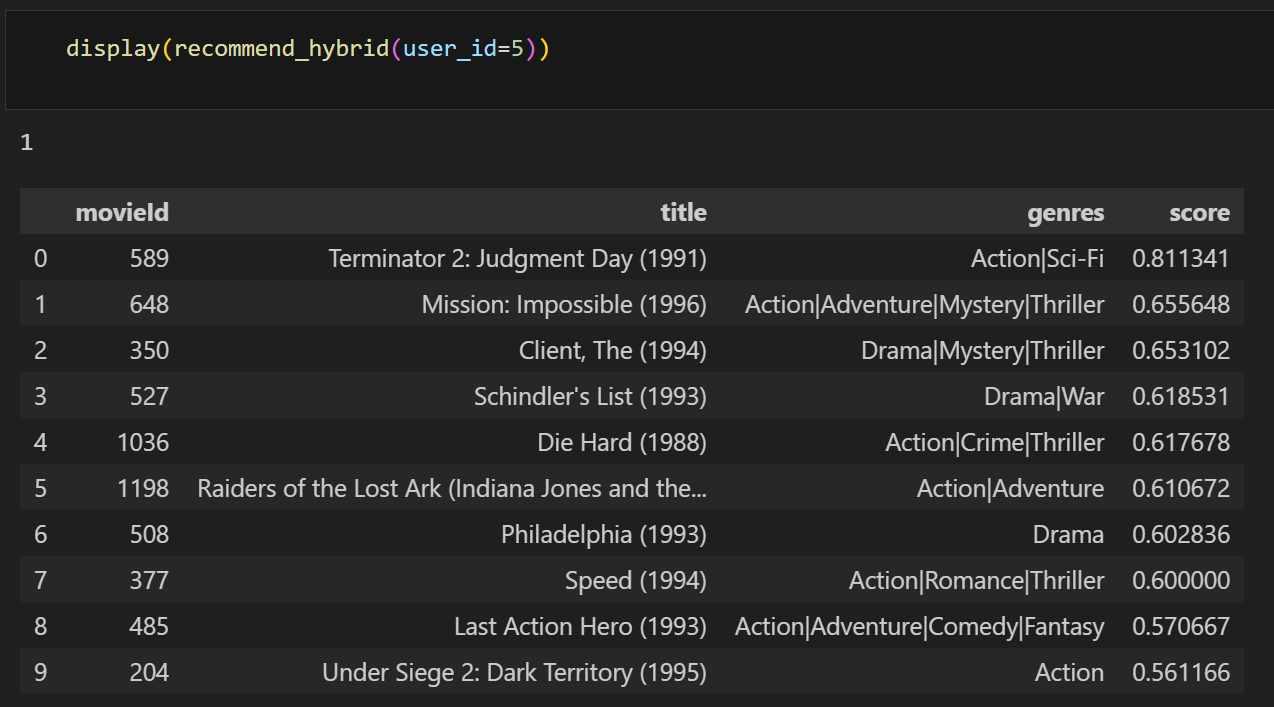
\includegraphics[width=1\textwidth]{pictures/results.png}
\caption{Rekomendacje filmów dla użytkownika o ID 5}
\label{fig:results}
\end{figure}

\section{Wnioski}
W przedstawionym projekcie stworzono i przeanalizowano system rekomendacyjny dla wypożyczalni filmów. W ramach prac wykonano pełną eksploracyjną analizę danych, zaprojektowano dwa niezależne modele rekomendacyjne – content-based filtering (CBF) oraz collaborative filtering (CF), a następnie zintegrowano je w systemie hybrydowym.

Na podstawie przeprowadzonych eksperymentów i analiz sformułowano następujące wnioski:
\begin{itemize}
    \item Dane wejściowe (oceny, tagi, gatunki) cechują się odpowiednią jakością i ilością, umożliwiającą efektywne tworzenie modeli rekomendacyjnych.
    \item Content-based filtering pozwala na precyzyjne profilowanie użytkownika w oparciu o jego preferencje gatunkowe i tematyczne, jednak jego skuteczność może być ograniczona w przypadku nowych użytkowników lub filmów bez wystarczających metadanych.
    \item Collaborative filtering, dzięki wykorzystaniu informacji o zachowaniach innych użytkowników, cechuje się wysoką skutecznością, lecz cierpi na tzw. problem zimnego startu.
    \item Wprowadzenie rozmytości w interpretacji podobieństwa (np. poprzez podobieństwo cosinusowe w skali $[0,1]$) pozwala modelować niepewność rekomendacji i lepiej dopasować wyniki do rzeczywistych preferencji użytkownika.
    \item System hybrydowy, łączący zalety obu podejść i odpowiednio je ważony, osiąga lepsze rezultaty niż pojedyncze komponenty, oferując bardziej trafne i stabilne rekomendacje.
\end{itemize}

Zrealizowany projekt potwierdza, że połączenie klasycznych metod rekomendacyjnych z podejściem rozmytym oraz analizą treści może prowadzić do skutecznego i elastycznego systemu rekomendacyjnego, gotowego do dalszego rozwoju i adaptacji.

\end{document}